\documentclass[dvipdfmx,10pt,a4paper,titlepage]{jsarticle}
\usepackage[dvipdfmx]{graphicx}
\usepackage{ascmac}
\usepackage{amsmath}
\usepackage{fancybox}
\usepackage{amssymb}
\usepackage{mathtools}
\usepackage{latexsym}
\usepackage{listings,jvlisting}
\usepackage{color}
\usepackage{url}
\definecolor{OliveGreen}{rgb}{0.0,0.6,0.0}
\definecolor{Orenge}{rgb}{0.89,0.55,0}
\definecolor{SkyBlue}{rgb}{0.28,0.28,0.95}
\lstset{
  language=C,
  basicstyle={\ttfamily},
  identifierstyle={\small},
  commentstyle={\small\itshape},
  keywordstyle={\small\bfseries},
  ndkeywordstyle={\small},
  stringstyle={\small\ttfamily},
  frame={tb},
  breaklines=true,
  columns=[l]{fullflexible},
  numbers=left,
  xrightmargin=0zw,
  xleftmargin=3zw,
  numberstyle={\scriptsize},
  stepnumber=1,
  numbersep=1zw,
  lineskip=-0.5ex,
  keepspaces=true,
  keywordstyle={\color{SkyBlue}},
  commentstyle={\color{OliveGreen}},
  stringstyle=\color{Orenge},
  showstringspaces=false
}
\title{電気電子情報実験・演習第二 課題12\\「FPGAを用いたアルゴリズム実装」最終レポート}
\author{電子情報工学科3年 03230422 佐藤 龍吾}
\date{\today}

\begin{document}
\maketitle
\section{実験の目的・背景}
本実験では、ハードウエア記述言語を用いてアルゴリズムを実装し、FPGA上で実行させることを目標とした。
現在、汎用プロセッサの性能は伸び悩みつつある。クロック周波数や集積度を上げることで性能を向上させることは難しくなってきていて、
近年はGPU (Graphic Processing Unit) など特定の処理に特化したデバイスを用いるアプローチが大きな成果を上げている。
FPGAはそのようなデバイスの一つであり、ハードウエア記述言語を用いて回路を記述・合成することで、特定の問題に特化したデバイスを作成することができる。

FPGAのようなハードウエア実装では、ソフトウエア実装にくらべ並列度・クロック周波数などを比較的容易に調整することができる。
よって、適切な実装を行えば、CPUより高速に問題を解決できるポテンシャルがある。
今回の実験では、基本課題としてVerilog HDL・FPGAの動作を学んだ後に
自由課題として一つの問題に対してソフトウエア実装とハードウエア実装を行い、性能比較を行った。
その結果をもとに、ハードウエアの特性やソフトとの違いを理解し、ハードウエア実装のポテンシャルについて考察した。


\section{基本課題}
\subsection*{基本課題1}
\subsubsection*{実験内容}
\begin{itemize}
    \item 課題1-1: 配布資料にあるプログラムEXE1をQuartusでコンパイルし、FPGA上で実行した。
    \item 課題1-2: EXE1で実装されたルーレットプログラムを改変し、点灯パタンを変更した。
    \begin{enumerate}
        \item 7セグの複数のセグメントを点灯させた。
        \item ルーレットの回転方向が一定周期で時計周り・反時計回りを繰り返すようにした。
        \item 7セグの中央のセグメントを一定のリズムでチカチカさせた。
    \end{enumerate}
\end{itemize}
\subsubsection*{実験結果}
課題1-1, 1-2のそれぞれに対し、Quartusでのコンパイル時に回路規模(必要ロジック数)と最大動作クロック周波数を測定した。結果は以下の通りである。
//TODO

課題1-1 → 1-2で処理が少し複雑になったことによって、
\begin{itemize}
    \item 回路規模は大きく変化しなかった。
    \item 必要な多入力演算器の数が多くなった。
\end{itemize}

\subsection*{基本課題2}
\subsubsection*{実験内容}
配布資料にあるプログラムEXE2(電卓・リモコン制御プログラム)をQuartusでコンパイルし、FPGA上で実行した。
\subsubsection*{実験結果}
//TODO
\subsection*{基本課題3}
\subsubsection*{実験内容}
\begin{itemize}
    \item 課題3-1: 配布資料にあるプログラムEXE31(VGA出力プログラム)をQuartusでコンパイルし、FPGA上で実行した。
    \item 課題3-2: 3-1のプログラムから、出力されるパタンを細分化(8x8 →16x16)した。
    \item 課題3-3: 3-2のプログラムに加え、左上に自分の名前(Ryugo.S)と表示させた。
\end{itemize}
\subsubsection*{実験結果}
//TODO

\subsection*{基本課題4}
\subsubsection*{実験内容}
\begin{itemize}
    \item 課題4-1: 配布資料にあるプログラムEXE41(音声入出力プログラム)をQuartusでコンパイルし、FPGA上で実行した。
    \item 課題4-2: 配布資料にあるプログラムEXE42(周波数の倍化・半化プログラム)をQuartusでコンパイルし、FPGA上で実行した。
\end{itemize}
\subsubsection*{実験結果}
//TODO
\section{自由課題}
\subsection{スケジュールと実装内容}
まず、実験のスケジュールと実装内容を表\ref{tab:schedule}に示す。
\begin{table}
    \begin{center}
        \caption{実験のスケジュールと実装内容}\label{tab:schedule}
        \begin{tabular}{|c|c|c|} \hline
            日付 & 実装内容 & 備考 \\ \hline
            10/12 & Pythonで山登り法・焼き鈍し法プログラムを実装 &  \\ \hline
            10/16 & 乱数計算・距離計算モジュールを実装 &  \\ \hline
            10/17 & 近傍生成・山登り法モジュールを実装 &  \\ \hline
            10/19 & ロジックのバグ修正・テストベンチ上で山登り法完動 &  \\ \hline
            10/23 & 山登り法モジュールの並列化 &  \\ \hline
            10/24, 26, 27 & FPGA上でうまく動作しないバグの修正 &  \\ \hline
        \end{tabular}
    \end{center}
\end{table}
\ref{sec:goal}節で述べた目標のうち、1. 2. について実行し、FPGA上で山登り法を並列に実行することで高速に巡回セールスマン問題の局所探索法を求めることができた。
次項から、実装したハードウエアの構成・アルゴリズムを説明する。

\subsection{ハードウエア構成}
\begin{figure}
    \caption{ハードウエア構成}\label{fig:hardware}
    \begin{center}
        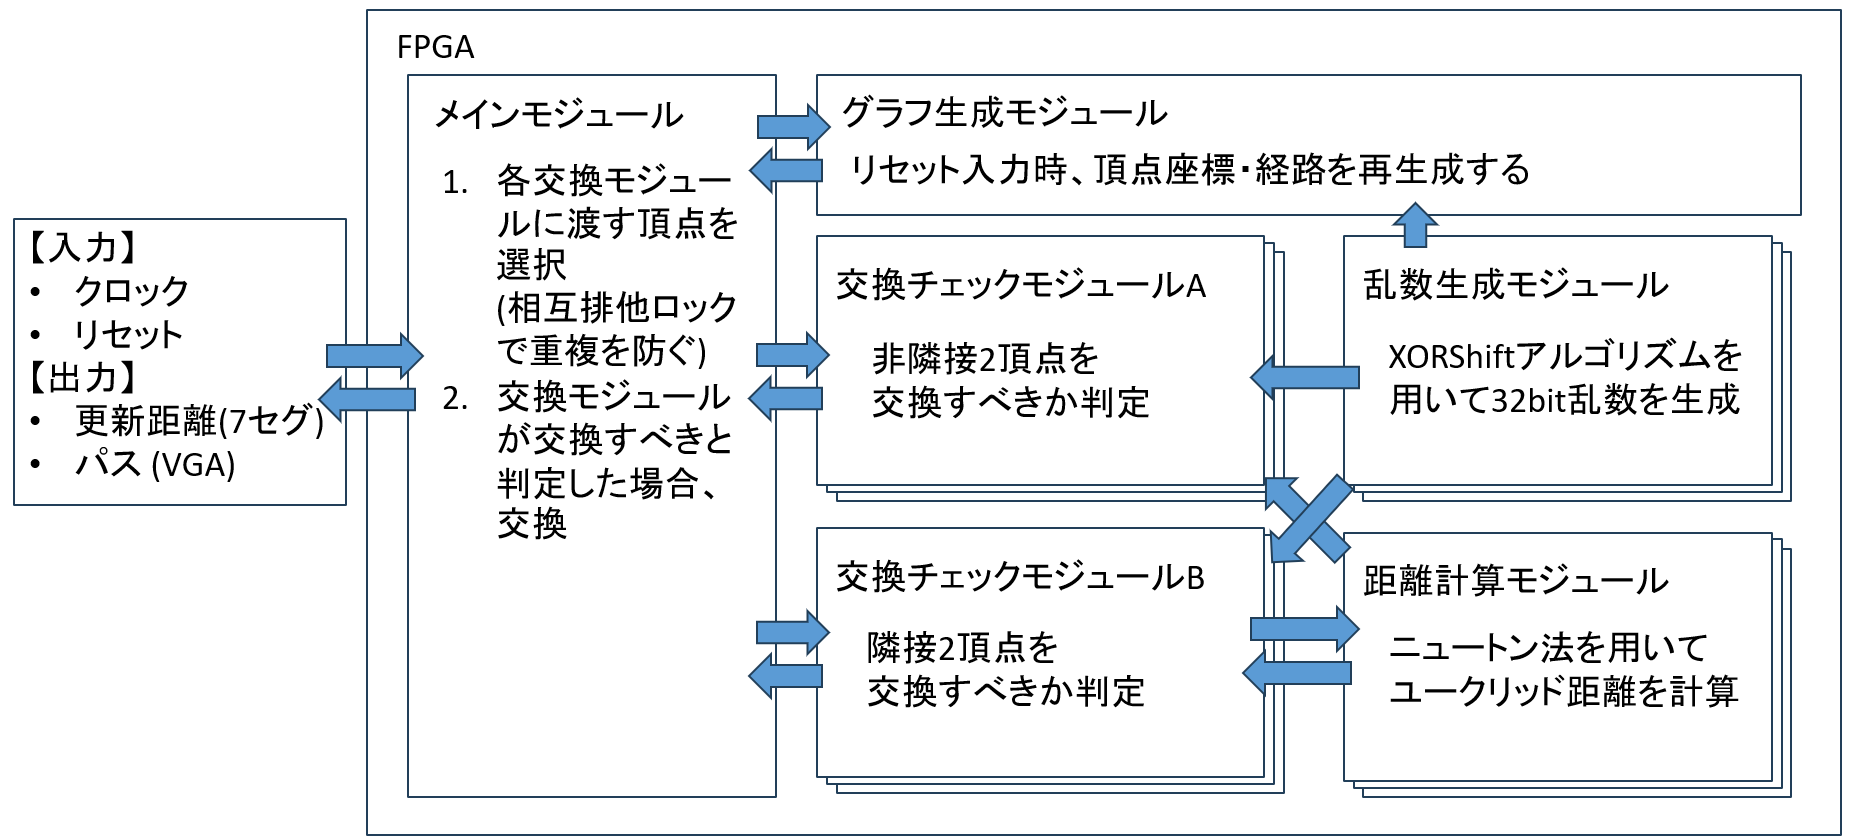
\includegraphics[width=15cm]{figure/hardware.png}
    \end{center}
\end{figure}

図~\ref{fig:hardware}にハードウエアの構成を示す。
FPGAには以下のモジュールを実装した。
\begin{itemize}
    \item メインモジュール(山登り法)
    \item グラフ生成モジュール(近傍生成)
    \item 交換チェックモジュール(交換判定)
    \item 乱数生成モジュール
    \item 距離計算モジュール
\end{itemize}
実行の流れは、
\begin{enumerate}
    \item リセット入力がなされると、グラフ生成モジュールが乱数生成モジュールを用いてランダムな頂点・経路を生成する
    \item メインモジュールが近傍を生成する。
    \item 交換チェックモジュールが距離計算モジュールを用いて交換の有無を判定する。
    \item メインモジュールが交換チェックモジュールからの結果を受け取り、交換の有無に応じて経路を更新する。
    \item 2. に戻る。
\end{enumerate}
である。2. ~ 4. は並列に実行される。

\subsection{乱数生成アルゴリズム}
今回の問題では、ランダムなグラフの生成・近傍の生成など、乱数を用いる箇所が多い。
FPGA上で疑似乱数を生成するためのアルゴリズムとして、今回はXORShiftを用いた。
XORShiftは状態$x, y, z, w$に対し、
\begin{align*}
    x \leftarrow& y \\
    y \leftarrow& z \\
    z \leftarrow& w \\
    w \leftarrow& (w\oplus(w>>19))\oplus((x\oplus(x<<11))\oplus((x\oplus(x<<11))>>8))
\end{align*}
を計算することで疑似乱数列${w}$を求めるアルゴリズムである。
ビット演算のみで計算できるため極めて高速で、また周期も$2^{128}-1$と非常に長く品質も高いという特徴がある。
このアルゴリズムを用いて、クロック毎に新しい乱数を生成するモジュールを作成し、乱数が必要な箇所それぞれでインスタンス化した。

\subsection{距離計算アルゴリズム}\label{sec:distance}
距離計算モジュールは、2つの頂点のx, y座標$(x_1, y_1), (x_2, y_2)$を受け取り、
2点のユークリッド距離$\sqrt{(x_1-x_2)^2+(y_1-y_2)^2}$を計算するモジュールである。

このモジュールでは、加算減算乗算に加え、平方根の計算が必要となるが、今回はニュートン法を用いて計算した。
ニュートン法において、$\sqrt{a}$の計算のためには、$f(x)=x^2-a$を考える。このとき、$f(x)=0$となる$x$が$\sqrt{a}$である。

解に近い値を初期値$x_0$とし、$x_{n+1}=x_n-\frac{f(x_n)}{f'(x_n)}=x_n-\frac{x_n^2-a}{2x_n}=\frac{x_n}{2}+\frac{a}{2x_n}$に従って$x_n$を更新していくと、
$x_n$は$\sqrt{a}$に収束していく。
今回はユークリッド距離の計算であり、初期値としてマンハッタン距離$d_m=|x_1-x_2|+|y_1-y_2|$を用いると、比較的早く収束する。
x座標、y座標が$[0,255]$の2点に対し、整数範囲で誤差1以内の距離を計算するには、$x_3$まで計算すれば十分であることがCPUプログラムによる検証により判明した。

当初、1クロックで$x_3$までの計算(二乗距離・マンハッタン距離・ニュートン法3回)を実行していたが、後述の通り周波数が大きく低下してしまったため、図~\ref{fig:distance}のように5クロックに分割しパイプライン化した。

\begin{figure}
    \begin{center}
        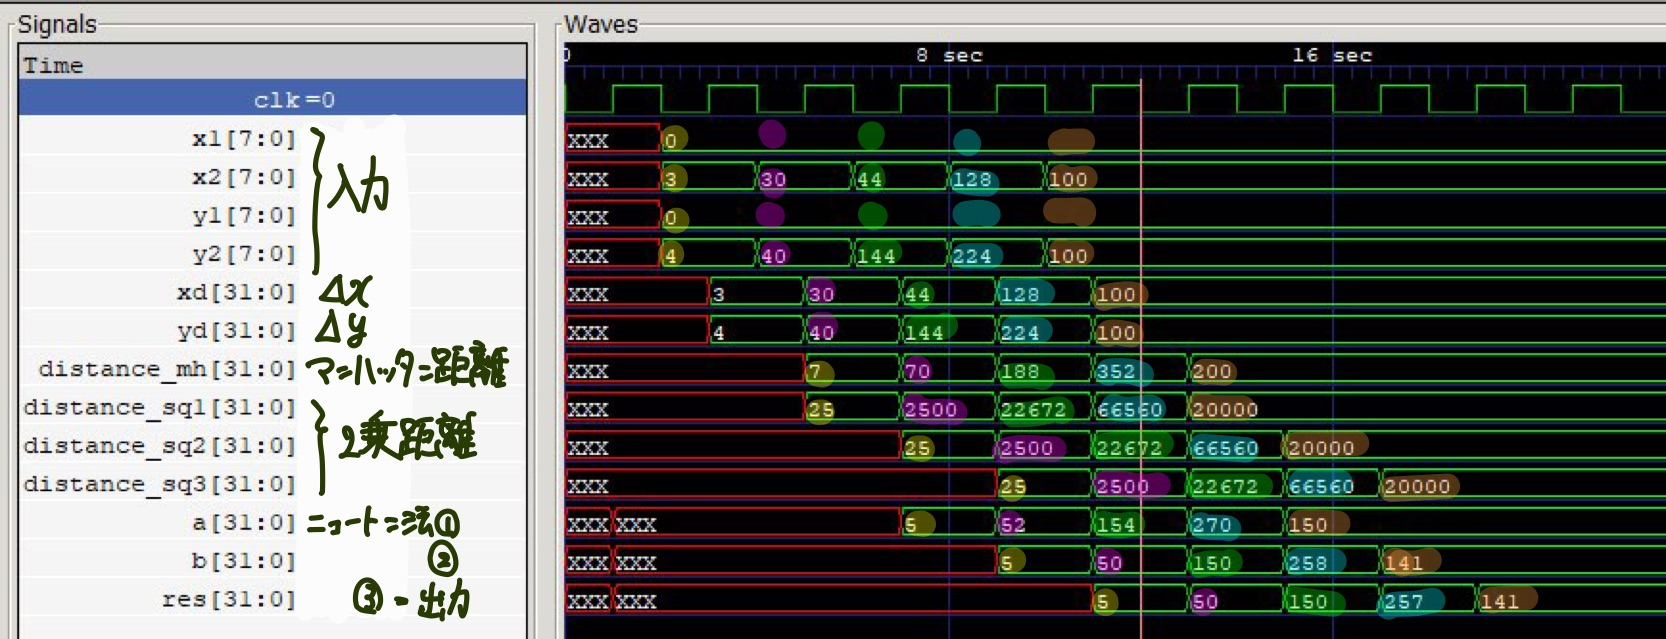
\includegraphics[width=15cm]{figure/distance_newton.jpg}
        \caption{距離計算モジュールのパイプライン化}\label{fig:distance}
    \end{center}
\end{figure}

\subsection{近傍生成アルゴリズム}
\ref{sec:local}節で述べたように、今回は経路の2点を入れ替えることで近傍を生成する。
交換する2点を選ぶには、交換する2点と、それぞれの前後の点の計6点の情報が必要であり、これら6点が重複しないように選択すれば、複数の箇所について同時に近傍を生成し、判定・更新を行うことができる。

各モジュールが頂点を選択する際は、以下の手順で行う
\begin{enumerate}
    \item 乱数生成モジュールから、頂点番号を表す[0,63]の乱数を2つ受け取り、$v_1, v_2$とする。
    \item ロック配列(後述)の$v_1-1, v_1, v_1+1, v_2-1, v_2, v_2+1$番目の要素を確認し、いずれも他のモジュールによってロックされていなければ、ロックを試みる。
    \item 再び$v_1-1, v_1, v_1+1, v_2-1, v_2, v_2+1$番目の要素を確認し、いずれもロックできていれば、交換チェックモジュールに6頂点の座標を送信する。
          一つ以上の頂点がロックに失敗していれば、6頂点すべてのロックを解除し、1. に戻る。
\end{enumerate}
ロック配列は、各頂点が他のモジュールによってロックされているかどうかを表す配列である。(ロックされていなければ-1, ロックされていれば、ロックしているモジュールのIDが格納される。)
この機能によって、複数のモジュールが同時に同じ頂点を選択することを防ぐことができる。
この手法は排他制御ロックと呼ばれており、データベースのトランザクション処理や、マルチスレッドプログラミングにおいてよく用いられる。

\subsection{交換判定アルゴリズム}
交換判定モジュールは、選択した2頂点(p,q)とその前後の頂点の座標を受け取り、距離計算モジュールを用いて交換するべきかどうか(交換によって総距離が短くなるかどうか)を判定する。

\fbox{パターン1}\hspace{10pt}p,qが隣接していない場合、p, qと前後を含めた6点がa→p→bとc→q→dの順に並んでいるとして、pとqを交換するので、
\begin{itemize}
    \item 交換前: $d(a,p)+d(p,c)+d(d,q)+d(q,f)$
    \item 交換後: $d(a,q)+d(q,c)+d(d,p)+d(p,f)$
\end{itemize}
の2つの距離を計算し、交換後の方が短ければ交換する。

\fbox{パターン2}\hspace{10pt}p,qが隣接している場合、p, qと前後を含めた4点がa→p→q→bの順に並んでいるとして、pとqを交換するので、
\begin{itemize}
    \item 交換前: $d(a,p)+d(p,q)+d(q,f)$
    \item 交換後: $d(a,q)+d(q,p)+d(p,f)$
\end{itemize}
を比較する。$d(p,q)=d(q,p)$より$d(a,p)+d(q,f)$と$d(a,q)+d(p,f)$を計算し、後者の方が小さければ交換する。

山登りモジュールではパターン1とパターン2をそれぞれいくつか用意し、並列度を上げた。


\section{参考文献}
\bibliography{source/FPGA} %hoge.bibから拡張子を外した名前
\bibliographystyle{junsrt} %参考文献出力スタイル
\end{document}